\documentclass[zavrsnirad]{fer}
% Dodaj opciju upload za generiranje konačne verzije koja se učitava na FERWeb
% Add the option upload to generate the final version which is uploaded to FERWeb


\usepackage{blindtext}
\usepackage{listings}
\usepackage{hyperref}
\usepackage[dvipsnames]{xcolor}
\definecolor{darkgreen}{rgb}{0, 0.6, 0}

\lstdefinelanguage{CSharp}{
	language=[Sharp]C,
	morekeywords={
		abstract, as, base, bool, break, byte, case, catch, char, checked, class, const, continue,
		decimal, default, delegate, do, double, else, enum, event, explicit, extern, false, finally,
		fixed, float, for, foreach, goto, if, implicit, in, int, interface, internal, is, lock, long,
		namespace, new, null, object, operator, out, override, params, private, protected, public,
		readonly, ref, return, sbyte, sealed, short, sizeof, stackalloc, static, string, struct, switch,
		this, throw, true, try, typeof, uint, ulong, unchecked, unsafe, ushort, using, virtual, void,
		volatile, while, async, await, var, dynamic
	},
	sensitive=true,
	morecomment=[l]{//},
	morecomment=[s]{/*}{*/},
	morestring=[b]",
}

\lstdefinelanguage{GraphQL}{
	keywords={
		query, mutation, subscription, type, input, interface, union, scalar, enum, fragment, on,
		implements, extend, schema, directive, extends, null, true, false
	},
	keywordstyle=\color{blue}\bfseries,
	ndkeywords={
		__schema, __type, __typename, __directive, __inputValue, __field, __enumValue, __typeKind
	},
	ndkeywordstyle=\color{violet}\bfseries,
	sensitive=true,
	morecomment=[s]{""" }{ """},
	morecomment=[s]{"""}{"""},
	morestring=[b]{"},
	morestring=[s]{"""}{"""}
}

\lstdefinelanguage{Javascript}{
	keywords={typeof, new, true, false, catch, function, return, null, catch, switch, var, if, in, while, do, else, case, break},
	keywordstyle=\color{blue}\bfseries,
	ndkeywords={class, export, boolean, throw, implements, import, this, static, async},
	ndkeywordstyle=\color{purple}\bfseries,
	identifierstyle=\color{black},
	sensitive=false,
	comment=[l]{//},
	morecomment=[s]{/*}{*/},
	commentstyle=\color{purple}\ttfamily,
	stringstyle=\color{red}\ttfamily,
	morestring=[b]',
	morestring=[b]"
}

\lstset{
	basicstyle=\ttfamily,
	keywordstyle=\color{blue}\bfseries,
	commentstyle=\color{darkgreen}\itshape,
	stringstyle=\color{red},
	showstringspaces=false,
	numberstyle=\tiny\color{gray},
	numbersep=5pt,
	tabsize=2,
	breaklines=true,
	showtabs=false,
	showspaces=false,
	showlines=true,
	frame=single,
	backgroundcolor=\color{lightgray}
}

%--- PODACI O RADU / THESIS INFORMATION ----------------------------------------

% Naslov na engleskom jeziku / Title in English
\title{GraphQL-based server monitoring system}

% Naslov na hrvatskom jeziku / Title in Croatian
\naslov{Sustav za praćenje stanja poslužitelja temeljen na jeziku GraphQL}

% Broj rada / Thesis number
\brojrada{1234}

% Autor / Author
\author{Dominik Dejanović}

% Mentor 
\mentor{Prof.\@ Ivana Bosnić}

% Datum rada na engleskom jeziku / Date in English
\date{June, 2024}

% Datum rada na hrvatskom jeziku / Date in Croatian
\datum{lipanj, 2024.}

%-------------------------------------------------------------------------------


\begin{document}


% Naslovnica se automatski generira / Titlepage is automatically generated
\maketitle


%--- ZADATAK / THESIS ASSIGNMENT -----------------------------------------------

% Zadatak se ubacuje iz vanjske datoteke / Thesis assignment is included from external file
% Upiši ime PDF datoteke preuzete s FERWeb-a / Enter the filename of the PDF downloaded from FERWeb
\zadatak{hr_0036541578_73-1.pdf}


%--- ZAHVALE / ACKNOWLEDGMENT --------------------------------------------------

\begin{zahvale}
  % Ovdje upišite zahvale / Write in the acknowledgment
  Hvala na kavi...
\end{zahvale}


% Odovud započinje numeriranje stranica / Page numbering starts from here
\mainmatter


% Sadržaj se automatski generira / Table of contents is automatically generated
\tableofcontents


%--- UVOD / INTRODUCTION -------------------------------------------------------
\chapter{Uvod}
\label{pog:uvod}


%-------------------------------------------------------------------------------
\chapter{Opis problema}
\label{pog:opis_problema}


%-------------------------------------------------------------------------------
\chapter{Korištene tehnologije}
\label{pog:koristene_tehnologije}
U ovom projektu su korištene razne tehnologije: RDBMS, web framework, backend tehnologije te brojne druge. U nastavku slijedi opis korištenih tehnologija.
\section{GraphQL}
GrapQL je jezik korišten za dohvaćanje i slanje podataka na API. Odabran je GraphQL umjesto REST tehnologije zbog nekoliko prednosti koje GraphQL ima:
 \begin{itemize}
 	\item ugrađena validacija polja - ovo omogućava GraphQL-u da provjeri polja koja korisnik unosi tako da se ne treba ručno programirati provjeravanje polja (na primjer GraphQL će automatski izbaciti grešku ukoliko se u brojčano polje unese znakovni niz). Također podcrtava pogreške prilikom korištenja nepoznatih parametara i polja
 	\begin{lstlisting}[language=GraphQL]
 		# INVALID: hero is not a scalar, so fields are needed
 		{
 			hero
 		}
 	\end{lstlisting}
 	\begin{lstlisting}[language=GraphQL]
 		{
 			"errors": [
 			{
 				"message": "Field \"hero\" of type \"Character\" must have a selection of subfields. Did you mean \"hero { ... }\"?",
 				"locations": [
 				{
 					"line": 3,
 					"column": 3
 				}
 				]
 			}
 			]
 		}
 	\end{lstlisting}
    \textcolor{red}{ADD REFERENCE TO https://graphql.org/learn/validation/}
 	\item upiti slični SQL-u - za razliku od REST-a koji se oslanja na putanje, GraphQL koristi Query kako bi korisnik mogao pomoću određenih parametara filtirati podatke te odabrati koje točno podatke želi dohvatiti
 	\item dohvaćanje više podataka u jednom zahtjevu - koristeći REST, korisnik bi morao za dohvaćanje raznih podataka slati puno upita, dok se u GraphQL-u može dohvatiti proizvoljan broj nepovezanih podataka u jednom zahtjevu
 	\begin{lstlisting}
 		{
 			empireHero: hero(episode: EMPIRE) {
 				name
 			}
 			jediHero: hero(episode: JEDI) {
 				name
 			}
 		}
 	\end{lstlisting}
 	\begin{lstlisting}[language=GraphQL]
 		{
 			"data": {
 				"empireHero": {
 					"name": "Luke Skywalker"
 				},
 				"jediHero": {
 					"name": "R2-D2"
 				}
 			}
 		}
 	\end{lstlisting}
 	\textcolor{red}{ADD REFERENCE https://graphql.org/learn/queries/}
 \end{itemize}

\section{HotChocolate}
\label{pog:hotchocolate}
HotChocolate je implementacija GraphQL poslužitelja u C\# programskom jeziku. Ona nam omogućava korištenje svih funkcionalnosti GraphQL tehnologije bez da ih moramo ručno implementirati.\\Korištena verzija: 13.6.0
\begin{figure}[htb]
	\centering
	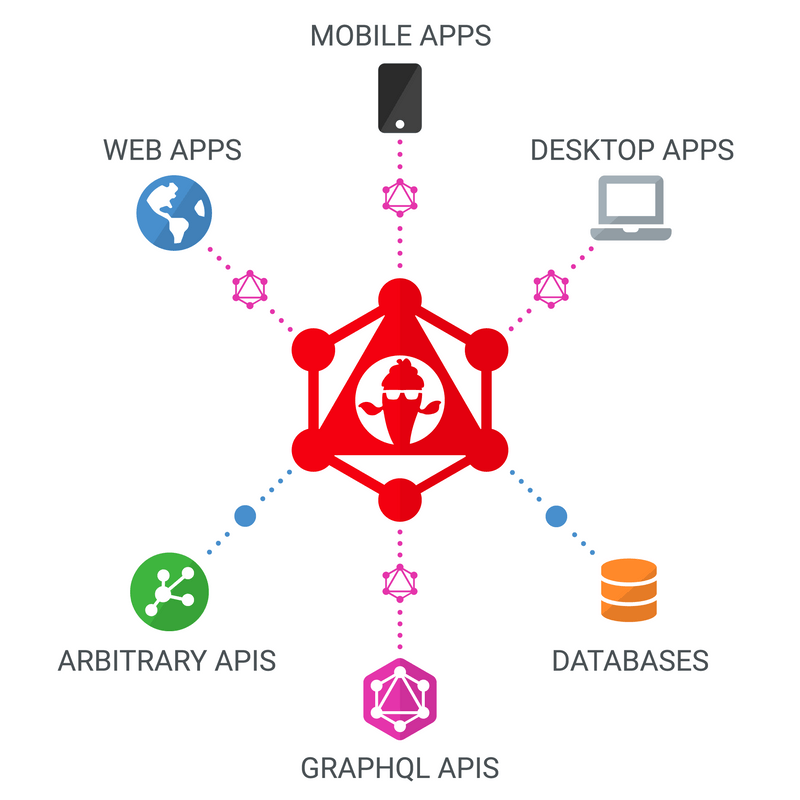
\includegraphics[width=0.6\linewidth]{images/hot_chocolate.png} 
	\caption{HotChocolate server}
	\label{slk:hot_chooclate}
\end{figure}
\\\textcolor{red}{ADD IMAGE REFERENCE} https://chillicream.com/static/cfd2ddde71f95ed876541f87c15b2a08/78d47/platform.png\\https://chillicream.com/docs/hotchocolate/v13

\section{.NET i C\#}
Za programiranje API-a i Monitor-a se koristi C\# programski jezik i .NET framework.\\
Korištena .NET verzija: net8.0\\Korištena C\# verzija: 12.0

\section{linq2db}
\label{pog:linq2db}
linq2db paket se koristi za pretvaranje LINQ koda u SQL kod kako bi se moglo lako pristupati bazi podataka.
\\Nakon instalacije paketa se pomoću određenih naredbi može spojiti na bazu podataka i iz nje generirati C\# klase koje odgovaraju tablicama u bazi podataka:
\begin{lstlisting}[language=CSharp]
	using System;
	using LinqToDB.Mapping;
	
	[Table("Products")]
	public class Product
	{
		[PrimaryKey, Identity]
		public int ProductID { get; set; }
		
		[Column("ProductName"), NotNull]
		public string Name { get; set; }
		
		[Column]
		public int VendorID { get; set; }
		
		[Association(ThisKey = nameof(VendorID), OtherKey=nameof(Vendor.ID))]
		public Vendor Vendor { get; set; }
		
		// ... other columns ...
	}
\end{lstlisting}
linq2db repozitorij: \url{https://github.com/linq2db/linq2db}

\section{Newtonsoft.Json}
Koristi se za serijalizaciju i deserijalizaciju JSON podataka.
Newtonsoft.Json repozitorij: https://github.com/JamesNK/Newtonsoft.Json

\section{Vue.js}
\label{pog:vue}
Vue.js je Javascript framework, koristi se za jednostavniji rad sa prikazom podataka i za bolje strukturiranje koda.
Primjer Vue koda za povećanja vrijednosti gumba nakon klika:
\begin{lstlisting}[language=html]
	<div id="app">
	<button @click="count++">
	Count is: {{ count }}
	</button>
	</div>
\end{lstlisting}
\textcolor{red}{ADD CODE REFERENCE TO https://vuejs.org/guide/introduction.html}
\\Vue.js dokumentacija: \url{https://vuejs.org/guide/introduction.html}

\subsection{vue-chartjs}
\label{pog:chart.vue}
\textcolor{red}{DOVRSI OVO}
\\Dokumentacija: https://vue-chartjs.org

\subsection{vue-collapsible-panel}
\label{pog:vue_collapsible_panel}
\textcolor{red}{DOVRSI OVO}
\\Dokumentacija: https://github.com/dafcoe/vue-collapsible-panel

\section{PostgreSQL}
Odabran je PostgreSQL kao RDBMS sustav za upravljanje bazom podataka zato što je otvorenog koda te ima opširnu dokumentaciju i korisničku podršku.
\\PostgreSQL dokumentacija: \url{https://www.postgresql.org/docs}

\section{Git}
Git je korišten kao sustav za praćenje verzija koda.
\\Službena git stranica: \url{https://git-scm.com}


%-------------------------------------------------------------------------------
\chapter{Opis rješenja}
\label{pog:opis_rjesenja}
Napravljene su tri .NET projekta, jedan Vue projekt te baza podataka. Slijedi detaljan opis svih aplikacija.

\section{Baza podataka}

\section{API}
API aplikacija je implementirana koristeći \ref{pog:hotchocolate} HotChocolate server paket koji implementira funkcionalnosti GraphQL.
\\Struktura projekta:
\textcolor{red}{SLIKA STRUKTURE}

\subsection{Program.cs}
Program.cs je datoteka koja se pokreće prilikom pokretanja programa. Glavne funkcije koje ona izvršava su konfiguracija Dependency Injectiona te mapiranje putanja API-a.
\textcolor{red}{ADD CODE}

\subsection{Query.cs}
\label{pog:query.cs}
Koristi se za dohvat podataka iz baze podataka. Za svaki tip podatka (CPU, memorija, tvrdi disk, ...) je napravljena metoda koja se poziva kada korisnik šalje zahtjev pomoću kojega se pokušava dohvatiti određen podatak. Primjer jedne takve metode:
\lstinputlisting[language=CSharp, title=Cpu metoda, firstline=20, lastline=49]{API/Query.cs}

\subsection{QueryHelper.cs}
Pomoćna klasa koju koristi \ref{pog:query.cs} Query.cs klasa. Sastoji se od raznih metoda od kojih je najbitnija GetLogs metoda koja sadržava algoritam koji se koristi za spajanje više podataka u jedan. Algoritam radi tako da pomoću početnog i zadnjeg datuma izračuna interval unutar kojeg se podaci spajaju u jedan:
\begin{lstlisting}[language=CSharp, title=Izračun intervala]
return (int)((DateTime)endDate).Subtract((DateTime)startDate).TotalHours;
\end{lstlisting}

\lstinputlisting[language=CSharp, title=Parametri GetLogs metode, firstline=97, lastline=104]{API/QueryHelper.cs}

\subsection{Db direktorij}
Db direktorij sadržava sve pomoćne klase i modele koji se koriste za interakciju sa bazom podataka. Većina klasa u direktoriju Models su automatski generirane (i djelomično ručno promijenjene) korištenjem \ref{pog:linq2db} linq2db paketa pomoću naredbe \textcolor{red}{SCAFFOLD}
\\Neke od važnijih klasa (te one koje nisu automatski generirane):
\begin{itemize}
	\item Models/IDb.cs - sučelje koje sadržava popis svih tablica u bazi podataka \textcolor{red}{ADD IMAGE}
	\item DatasetHelper.cs - pomoćna klasa korištena u algoritmu spajanja više podataka u jedan podatak \textcolor{red}{REFERENCE NA ALGORITAM}
	\item MonitoringDb.cs - automatski generirana implementacija IDb.cs sučelja
	\item MonitoringDbProvider.cs - koristi se za generiranje nove konekcije na bazu podataka (potrebno jer se koristi Dependency Injection)
\end{itemize}

\subsection{Mutations direktorij}
Sadržava klase i sučelja koja se koriste za dodavanje i osvježavanje podataka u bazi podataka.
\\Važnije klase i sučelja u direktoriju:
\begin{itemize}
	\item IMutationHelper - sučelje koje definira funkcionalnosti koje su potrebne za umetanje, osvježavanje i brisanje pojedinačnih ili liste podataka iz baze podataka \textcolor{red}{ADD PIC OF INTERFACE}
	\item MutationHelper - implementacija IMutationHelper sučelja
\end{itemize}
Primjer dijela jedne mutacije:
\lstinputlisting[language=CSharp, firstline=10, lastline=24, title=CpuMutation.cs]{API/Mutations/CpuMutation.cs}

\subsection{Konfiguracijske datoteke}
U programu se nalaze tri konfiguracijske datoteke: appsetting.json, appsettings.Development.json i dbConnectionString.txt od kojih će samo zadnja biti opisana.
\\dbConnectionString.txt datoteka sadržava niz znakova koji se koristi za spajanje na postojeću bazu podataka prilikom pokretanja programa:
\begin{lstlisting}[title=dbConnectionString.txt]
	Host=localhost;Username=[username];Password=[password];Database=[dbName];Include Error Detail=[true for debugging; false for deployment]
\end{lstlisting}

\subsection{Pokretanje API-a}
API se pokreće iz komandne linije/terminala pomoću naredbe "dotnet run" unutar direktorija u kojem se API nalazi.
\\Nakon pokretanja se može pristupiti URL-u \url{http://localhost:3000//graphql}, prilikom čega se otvara web stranica na kojoj se može vidjeti dokumentacija API-a te se mogu izvršavati upiti.
\begin{figure}[!htb]
	\centering
	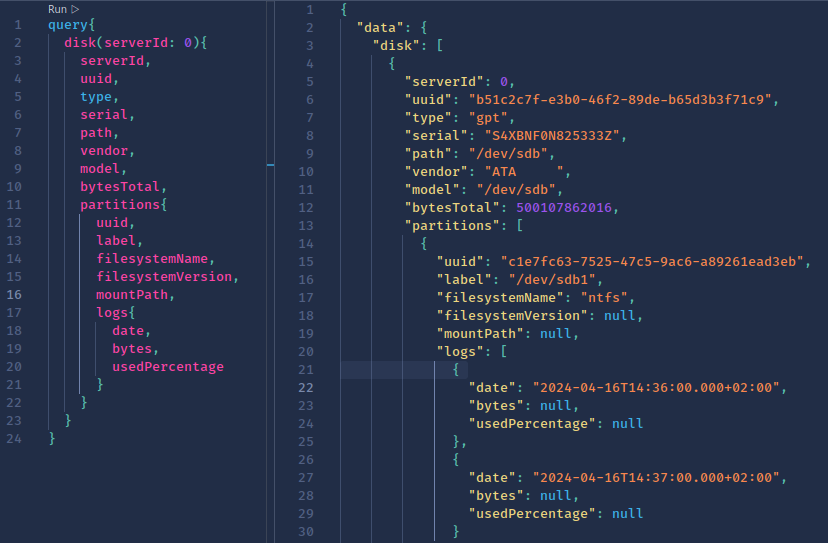
\includegraphics[width=1\linewidth]{images/api_query.png} 
	\caption{Dohvat podataka o pohrani}
	\label{slk:api_query}
	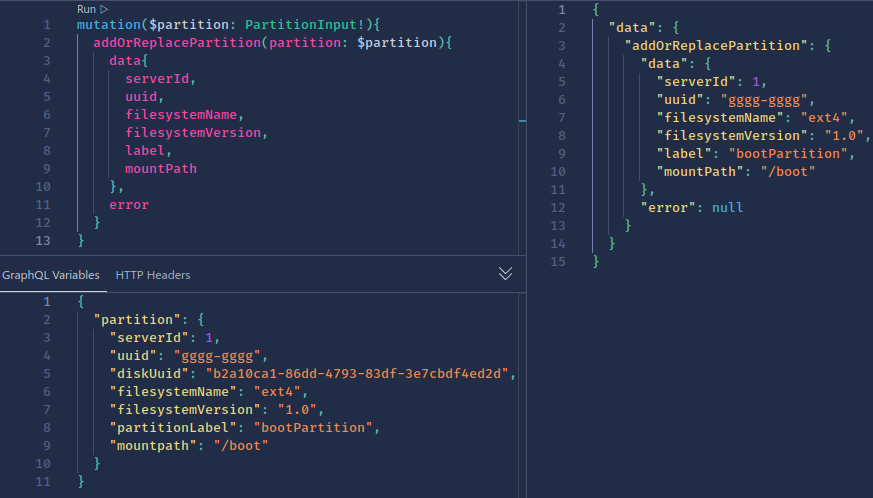
\includegraphics[width=1\linewidth]{images/api_mutation.png} 
	\caption{Dodavanje jedne particije}
	\label{slk:api_mutation}
\end{figure}

\section{Monitor}
Aplikacija Monitor se koristi za prikupljanje podataka o poslužitelju te slanje tih podataka API-u.
\\Struktura aplikacije: \textcolor{red}{ADD IMAGE}
\\Objašnjenje važnijih dijelova aplikacije
\begin{itemize}
	\item Monitor.cs - pokreće se prilikom pokretanja aplikacije
	\item Models direktorij - sadržava klase koje se koriste za serijalizaciju i deserijalizaciju podataka dohvaćenih sa terminala
	\item ApiHelper.cs - koristi se za slanje podataka API-u
	\item config.json - koristi ju korisnik kako bi konfigurirao aplikaciju
	\item DataHelper.cs - čita podatke sa terminala te ih deserijalizira u klase koje se nalaze u Models direktoriju
	\item LogHelper.cs - pokreće proces dohvaćanja podataka svakin [n] minuta (n = definiran u config.json datoteci)
	\item ProcessHelper.cs - koristi se za pokretanje procesa u terminalu
\end{itemize}

\subsection{Monitor.cs}
Pokreće se prilikom pokretanja aplikacija. Na početku učitava konfiguracijsku datoteku, te zatim pomoću beskonačnoj petlji pokreće proces prikupljanja podataka te slanje tih podataka API-u.
\lstinputlisting[firstline=10,lastline=30,language=CSharp]{Monitor/Monitor.cs}

\section{Common}
Projekt Common sadržava klase i sučelja koje koristi više projekata. Stvoren je kako bi se izbjeglo ponavljanje koda.
\textcolor{red}{ADD PICTURE}
Neke od važnijih klasa i sučelja:

\subsection{ILog.cs}
Glavno sučelje, svaki Log nasljeđuje polja definirana u njemu.

\subsection{Graphql direktorij}
Graphql direktorij sadržava klase i sučelja koji se koriste za komunikaciju API i Monitor programa.
Neko od važnijih komponenti direktorija:
\begin{itemize}
	\item Payload.cs - sastoji se od Data polja koje sadržava podatke o poslužitelju koji se vraćaju korisniku te Error polja koje je prazno osim u slučaju pogreške prilikom obrade zahtjeva
	\item InputModels direktorij - sadržava klase koje se koriste prilikom dodavanja ili izmijene podataka. Primjer klase:
	\lstinputlisting[firstline=3,language=CSharp,title=CpuInput.cs]{Common/Models/Graphql/InputModels/CpuInput.cs}
	\item Logs direktorij - sadržava klase koje opisuju Log podatke za određen aspekt poslužitelja
	\item OutputModels direktorij - sadržava klase koje se koriste prilikom vraćanja API odgovora. Primjer klase:
	\lstinputlisting[firstline=5,language=CSharp,title=MemoryOutput.cs]{Common/Models/Graphql/OutputModels/MemoryOutput.cs}
\end{itemize}

\section{Web stranica}
Web stranica je napravljena pomoću \ref{pog:vue} Vue frameworka, te se koriste \ref{pog:chart.vue} Chart.vue i \ref{pog:vue_collapsible_panel} vue-collapsible-panel paketi kako bi se prikazali podaci o poslužitelju.

\subsection{public/index.html}
Koristi se Vue framework te se zbog toga koristi samo jedna HTML stranica, u kojoj se prikazuju renderirane komponente.

\subsection{App.vue}
Glavna .vue datoteka koja kontrolira sadržaj koji se prikazuje, stvara se prilikom pokretanja programa.

\subsection{src/components direktorij}
Vue framework koristi komponente kako bi se dijelovi koda mogli ponovno koristiti. Sve komponente se nalaze u ovom direktoriju. Primjer dijela jedne takve komponente:
\lstinputlisting[language=Javascript,firstline=45,title=MemoryInfo.vue]{website/src/components/MemoryInfo.vue}

\subsection{src/models direktorij}
Models direktorij sadržava klase koje se koriste za pohranjivanje podataka dohvaćenih s API-a. Primjer klase:
\lstinputlisting[firstline=3,language=Javascript,title=Partition.ts]{website/src/models/Partition.ts}

\subsection{api.ts}
Zadužen za dohvaćanje podataka s API-a. Primjer dohvaćanja podataka o procesoru za trenutni server:
\lstinputlisting[title=getCpu(),firstline=27,lastline=53,language=Javascript]{website/src/api.ts}

\subsection{ChartHelper.ts}
Pomoćna datoteka koja se koristi za pretvorbu podataka koje API vraća u točke na grafu.

%--- LITERATURA / REFERENCES ---------------------------------------------------

% Literatura se automatski generira iz zadane .bib datoteke / References are automatically generated from the supplied .bib file
% Upiši ime BibTeX datoteke bez .bib nastavka / Enter the name of the BibTeX file without .bib extension
\bibliography{literatura}



%--- SAŽETAK / ABSTRACT --------------------------------------------------------

% Sažetak na hrvatskom
\begin{sazetak}
  Unesite sažetak na hrvatskom.
\end{sazetak}

\begin{kljucnerijeci}
  prva ključna riječ; druga ključna riječ; treća ključna riječ
\end{kljucnerijeci}


% Abstract in English
\begin{abstract}
  Enter the abstract in English.
  
\end{abstract}

\begin{keywords}
  the first keyword; the second keyword; the third keyword
\end{keywords}


%--- PRIVITCI / APPENDIX -------------------------------------------------------

% Sva poglavlja koja slijede će biti označena slovom i riječi privitak / All following chapters will be denoted with an appendix and a letter
\backmatter

\chapter{The Code}


\end{document}
